\documentclass[conference,10pt]{IEEEtran}
\IEEEoverridecommandlockouts
\usepackage{cite}
\usepackage{amsmath,amssymb}
\usepackage{newtxtext,newtxmath}
\usepackage{booktabs}
\usepackage{graphicx}
\renewcommand{\arraystretch}{0.90}
\setlength{\tabcolsep}{4pt}
\setlength{\textfloatsep}{5pt plus 1pt minus 1pt}
\setlength{\floatsep}{5pt plus 1pt minus 1pt}
\setlength{\intextsep}{5pt plus 1pt minus 1pt}
\setlength{\abovecaptionskip}{3pt}
\setlength{\belowcaptionskip}{1pt}

\begin{document}

\title{Efficient Uncertainty-Aware Neural Operator Forecasting of Experimental Airfoil Wakes}

\author{\IEEEauthorblockN{Aryamann Srivastava\textsuperscript{*}, Prashant Kumar, and Rajesh Ranjan}
\IEEEauthorblockA{Department of Aerospace Engineering\\
Indian Institute of Technology Kanpur, Kanpur, India\\
\textsuperscript{*}Student author, B.Tech. (Aerospace Engineering)}}

\maketitle

\begin{abstract}
Forecasting experimentally measured fluid flows with neural operators is challenging: the measurements are noisy, spatially incomplete and few, while deployment is constrained in memory and runtime. This work develops an efficient neural operator framework for multi-step forecasting of turbulent airfoil wakes from particle image velocimetry (PIV), together with spatially resolved prediction intervals. A fine-tuned Fourier Neural Operator (FNO) provides the point forecast, while a lightweight U-Net estimates forecast-dependent residual magnitude and a lookup-table calibration converts it into prediction intervals. Separating forecasting from uncertainty calibration permits interval refinement without modifying the point predictor: recalibration raises the interval-quality score by 5.2 points with the forecast held byte identical, and the complete system runs in 7.5\,s of a 300\,s budget inside a 256\,MB package. Experiments further show that constraints valid for the underlying three-dimensional flow can degrade prediction of planar PIV measurements, emphasizing the role of the measurement operator in physics-informed learning.
\end{abstract}

\begin{IEEEkeywords}
neural operators, scientific machine learning, uncertainty quantification, turbulent wakes, PIV
\end{IEEEkeywords}

\section{Introduction}
\textbf{Motivation.} Neural operators have emerged as efficient surrogates for PDE-governed flows~\cite{fno}. Our objective is to forecast a turbulent airfoil wake from particle image velocimetry (PIV) and return a calibrated uncertainty interval for every predicted value, inside a fixed memory and runtime budget. Experimental data makes this hard: measurements are noisy, observe only a plane of a three-dimensional flow, are few, and test conditions lie outside the training range.

\textbf{Limitations of prior work.} Operator-learning studies are largely developed and validated on clean simulation data, report accuracy without calibrated uncertainty, and assume an unconstrained inference budget; all three assumptions fail here. Physics-informed variants add PDE residuals to the loss, but those residuals are written for the latent flow rather than for what the instrument records. We break from this by treating uncertainty as a separately calibrated output, and by testing rather than assuming that latent-flow constraints apply to a planar measurement.

\textbf{Key insights and contributions.} Two insights enable the approach. Since the half-width enters only the bounds, uncertainty can be calibrated after the fact without retraining or perturbing the point forecast, so a frozen backbone and a tight memory budget cost nothing in calibration quality. And a constraint valid for the latent flow need not hold for the measured observable, which explains why several standard physics constraints actively hurt. The contributions are an efficient FNO--U-Net framework for forecasting and residual-based uncertainty from PIV, a decoupled interval calibration that refines uncertainty without changing the forecast, and a measurement-operator analysis of when physics constraints apply.

\textbf{Limitations of the proposed approach.} Calibration transfers across a distribution shift but the fluctuation correction does not, and conditioning the lookup table on spatial position improved calibration in-sample while degrading it out-of-sample, so richer conditioning needs a transfer-aware fit. Carrying the measurement-operator view into the training loss, instead of only using it to rule constraints out, is left to future work.

\section{Problem and Testbed}
The data and the evaluation protocol used here are those of the RealPDE Sim2Real benchmark~\cite{realpdebench}, released as part of a NeurIPS 2026 competition track; we adopt both unchanged as a standardised experimental testbed. Given 20 consecutive frames of a two-dimensional velocity field $(u,v)$ on a $32\times 64$ PIV grid behind a NACA~4418 airfoil, the objective is to predict the subsequent 20 frames and provide lower and upper bounds for every predicted scalar. The training set contains 81 experimental trajectories (69,085 frames), spanning $Re=3{,}750$--$26{,}700$ and angles of attack of $0^\circ$--$20^\circ$. Test conditions are unseen and extend beyond the training Reynolds-number range; neither $Re$ nor geometry is supplied to the model.

The package is limited to 256\,MB, including a 201.4\,MB pretrained FNO backbone, and inference must complete within 300\,s using PyTorch and NumPy. Evaluation combines five metrics: relative $L_2$ error of the velocity field (\texttt{rel\_l2}), of the turbulent kinetic energy field (\texttt{tke}), and of the mean velocity profile at nine downstream probes (\texttt{mvpe}), each mapped to a score by $100/(1+e/2)$; runtime, mapped by $100/(1+(t/728.96)^{1/2})$; and interval quality (\texttt{sps}), proportional to $\mathbb{E}[e^{-w/\sigma}\mathbf{1}(\text{covered})]$ with $\sigma=0.0564$, so that width is penalised exponentially and an interval missing its target scores zero. Interval quality carries about one quarter of the weight in the combined score, making uncertainty a first-class objective rather than a diagnostic.

\section{Design}
Figure~\ref{fig:pipeline} summarizes the framework. The FNO3d backbone is fine-tuned on the experimental trajectories. Since the memory budget permits only one backbone at inference, independently fine-tuned models are averaged in weight space~\cite{soup}, avoiding ensemble cost. Squared-error training produces an over-smoothed forecast retaining approximately 74\% of the true fluctuation energy; a lightweight auxiliary network rescales predicted fluctuations, improving \texttt{tke} by 2.21 points in isolation.

For uncertainty estimation, the input and predicted sequences are concatenated and supplied to a U-Net~\cite{unet}, which predicts a centre correction $c$ and a residual magnitude $|\hat r|$. The latter is mapped through a 24-bin lookup table to a spatially varying half-width $h$, giving the interval
\begin{equation}
[\hat y+\alpha c-h,\;\hat y+\alpha c+h].
\label{eq:interval}
\end{equation}
The widths in~\eqref{eq:interval} are calibrated directly from empirical residuals, following split conformal calibration~\cite{conformal} but with the quantile a learned function of the forecast rather than a global constant.

\begin{figure}[t]
\centering
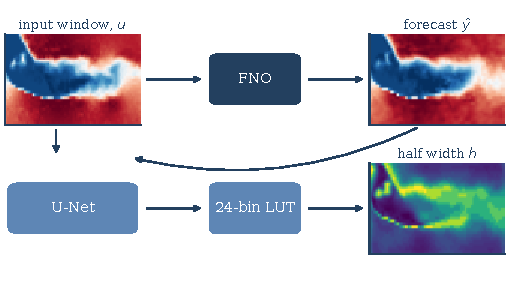
\includegraphics[width=0.88\columnwidth]{figure1_pipeline.pdf}
\caption{Resource-constrained forecasting and uncertainty pipeline. The FNO predicts the future sequence; a U-Net estimates forecast-dependent residual magnitude and centre correction, followed by lookup-table interval calibration. Contours show a held-out case at $Re=13{,}950$, $20^\circ$.}
\label{fig:pipeline}
\end{figure}

\section{Evaluation}

\begin{table}[t]
\caption{Component ablation on the development set.}
\label{tab:ablation}
\centering\small
\begin{tabular}{@{}lrrrr@{}}
\toprule
Configuration & \texttt{tke} & \texttt{sps} & Combined & $\Delta$\\
\midrule
Fine-tuned FNO (weight avg.) & 76.00 & 34.37 & 78.45 & --\\
\hspace{0.55em}+ U-Net interval head & 76.00 & 37.48 & 79.25 & $+0.80$\\
\hspace{0.55em}+ fluctuation correction & 78.62 & 38.29 & 79.59 & $+0.10$\\
\hspace{0.55em}+ interval width calibration & 78.62 & 39.56 & 80.06 & $+0.20$\\
\bottomrule
\end{tabular}
\end{table}

\begin{table}[t]
\caption{Scores on the development and held-out evaluation sets.}
\label{tab:results}
\centering\small
\begin{tabular}{lrr}
\toprule
Metric & Development & Held-out\\
\midrule
\texttt{rel\_l2} & 93.977 & 91.158\\
\texttt{tke} & 78.623 & 59.882\\
\texttt{mvpe} & 93.244 & 91.598\\
\texttt{time} & 90.771 & 78.952\\
\texttt{sps} & 39.558 & 53.847\\
\midrule
Combined & 80.081 & 75.087\\
\bottomrule
\end{tabular}
\end{table}

Table~\ref{tab:ablation} reports each cumulative configuration, $\Delta$ being the isolated effect of the added stage; backbone refinements lie between rows, so Combined is not the running sum of $\Delta$. Two of the largest single gains, $+0.80$ from the interval head and $+0.20$ from recalibrating the widths, were both obtained with the point forecaster held byte identical; the fluctuation correction contributes little to the combined score but supplies the entire 2.21-point gain in \texttt{tke}, the metric it targets. Optimising the inference path alone, by loading the checkpoint device-side and storing assets uncompressed, raised the score to the 80.081 of Table~\ref{tab:results} with no change to any model.

The same model scored 75.087 on the held-out set, at 7.5\,s and 51.8\,s of inference against a 300\,s limit.

We also tested three physically motivated constraints. A divergence-free prediction cost about 9 points, since 45\% of measured fluctuation energy was non-solenoidal. A momentum-residual loss was similarly ineffective: two-dimensional vorticity transport accounts for only 4--12\% of the observed temporal tendency. POD truncation removed fine-scale turbulence rather than measurement noise.

All three have a common interpretation. PIV measures a plane of a three-dimensional flow, $\mathbf{y}=\mathcal{M}(\mathbf{q})+\boldsymbol{\epsilon}$, with $\mathbf{q}$ the latent flow, $\mathcal{M}$ the measurement operator and $\boldsymbol{\epsilon}$ the noise. A constraint valid for $\mathbf{q}$ need not hold for $\mathbf{y}$, so physics-informed learning from experimental data must distinguish consistency of the latent system from consistency with the observable.

\section{Conclusion and Future Work}
We presented an efficient neural-operator framework for forecasting experimental airfoil wakes with spatially resolved uncertainty inside a 256\,MB memory and 300\,s runtime budget, in which separating point prediction from residual-based interval calibration replaces an inference-time ensemble.

Future work is to condition the interval width on a transfer-aware feature set, and to embed the measurement operator in the training loss rather than using it only to rule constraints out.

\section*{Acknowledgment}
Part of this work was carried out as a participating entry in Track~1 (Sim2Real) of the RealPDE challenge at NeurIPS 2026, from which the dataset and the evaluation metrics are taken. Portions of the text of this manuscript were drafted and edited with the assistance of a large language model~\cite{claude}. All models, experiments, measurements and analyses reported here are the authors' own.

\begin{thebibliography}{00}
\scriptsize\setlength{\itemsep}{-1pt}
\bibitem{fno} Z. Li \textit{et al.}, ``Fourier neural operator for parametric partial differential equations,'' in \textit{Proc. ICLR}, 2021.
\bibitem{realpdebench} Z. Hu \textit{et al.}, ``RealPDEBench: A benchmark for complex physical systems with real-world data,'' in \textit{Proc. ICLR}, 2026.
\bibitem{soup} M. Wortsman \textit{et al.}, ``Model soups: Averaging weights of multiple fine-tuned models improves accuracy without increasing inference time,'' in \textit{Proc. ICML}, 2022.
\bibitem{unet} O. Ronneberger, P. Fischer, and T. Brox, ``U-Net: Convolutional networks for biomedical image segmentation,'' in \textit{Proc. MICCAI}, 2015.
\bibitem{conformal} A. N. Angelopoulos and S. Bates, ``Conformal prediction: A gentle introduction,'' \textit{Found. Trends Mach. Learn.}, vol. 16, no. 4, 2023.
\bibitem{claude} Anthropic, ``Claude,'' large language model, 2026. [Online]. Available: https://claude.ai
\end{thebibliography}

\end{document}
